\documentclass[11pt,oneside,a4paper]{article}
\usepackage[utf8]{inputenc}
\usepackage{amsmath}
\usepackage{graphicx}
\usepackage[spanish]{babel}
\title{Memoria Práctica 1. Aplicación de PCA y LDA a OCR}
\author{Marcos Esteve Casademunt, Jose Gómez Gadea}
\date{Abril 2018}

\begin{document}

\maketitle
\tableofcontents
\listoffigures

\section{PCAExperiment}
Los resultados de este experimento son:

\begin{center}
\begin{tabular}{l c}
10 &	10.369 \\
20	 & 6.231 \\
30 &	5.434 \\
40	 & 4.935 \\
50	 & 5.184 \\
60 &	5.184 \\
70	 & 5.234 \\
80 &	5.334 \\
90 &	5.434 \\
100 & 	5.434 \\
\end{tabular}
\end{center}
\begin{figure}
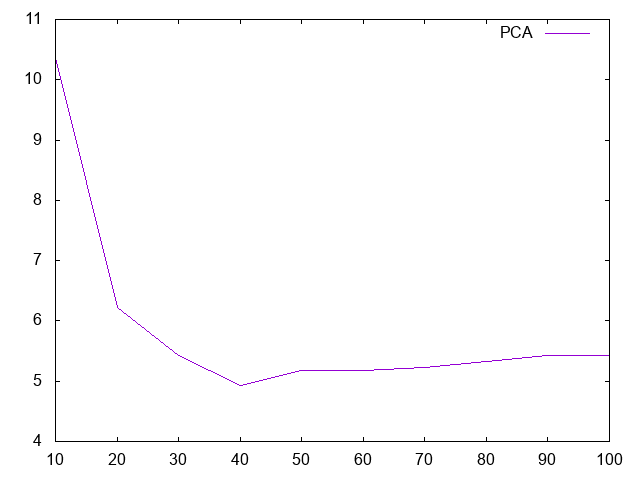
\includegraphics[scale=0.8]{salida.png}
\caption{Reducción de dimensionalidad usando PCA }
\end{figure}

Como podemos observar para una reducción a 40 dimensiones se obtiene un error de clasificación de 4,93\%

\section{LDAExperiment}
LDA únicamente proyecta hasta un máximo de C-1 dimensiones. Por ello, solo se podrá proyectar hasta un máximo de 9 dimensiones.

Los resultados son para PCA:

\begin{center}
\begin{tabular}{l c}
1 &	64.257\\
2 &	51.695\\
3 &	43.220\\
4 &	29.462\\
5 &	25.174\\
6 &	20.738\\
7 &	17.049\\
8	& 14.706\\
9	& 12.712\\
\end{tabular}
\end{center}


Y para LDA: 


\begin{center}
\begin{tabular}{l c}
1 &	57.777\\
2 &	45.513\\
3 &	38.584\\
4 &	23.779\\
5 &	16.650\\
6 &	13.759\\
7 &	12.812\\
8 &	11.466\\
9 &	11.117\\
\end{tabular}
\end{center}
\begin{figure}
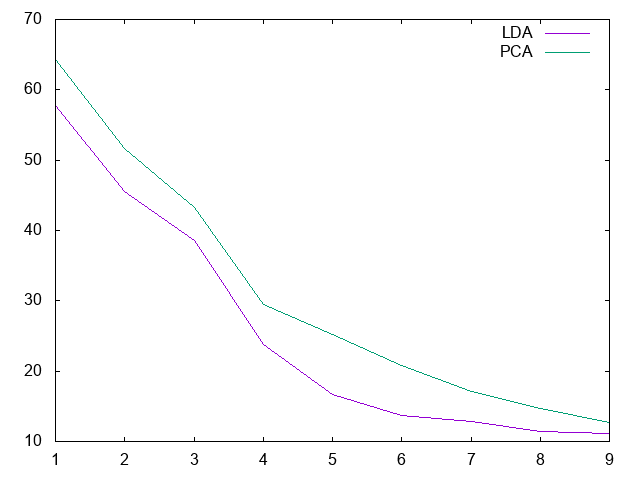
\includegraphics[scale=0.8]{salida2.png}
\caption{Reducción de dimensionalidad usando PCA VS LDA}
\end{figure}


Como podemos observar, LDA es mejor que PCA en el rango [1:9]. KNN obtiene buenos resultados con esta reducción, sobre un 89\% de acierto. Aunque, como hemos visto anteriormente, reduciendo con PCA a 40 dimensiones KNN obtiene una tasa de acierto del 95\% aproximadamente.

\end{document}
